\documentclass{article}
	\usepackage{natbib}
	\usepackage{booktabs}
	\usepackage{amsmath}
	\usepackage{graphicx}
	\usepackage{subcaption}
	\usepackage{hyperref}
	\usepackage{setspace}
	

\begin{document}

\title{Toward Intelligent Political Actors}
	\author{David Masad}
	\maketitle
\onehalfspacing
\section{Introduction}
The model presented by \citet{axelrod_1997}, commonly known as the Tribute Model, is an early example of what \citet{epstein_1996} refer to as `artificial societies' -- agent-based models in which simple rules lead to the emergence of phenomena with recognizable real-world analogue. Agents in the Tribute Model represent atomic geopolitical actors, interacting with each other via demands for tribute (hence the model's name) which are responded to with either payment or war. Past interactions may yield future cooperation, leading to the emergence of stable blocs of agents acting together against rival blocs. A similar approach was used by Axelrod's student Lars-Erik Cederman in the GeoSim family of models \citep{cederman_2003}, also with rich results.

Both Axelrod and Cederman's agents use simple heuristics to decide whether to go to war. While it is the case that many features of the international system emerge from agents using such heuristics, they are nevertheless a major departure of the models from both empirical evidence and qualitative theories of state behavior. Even ancient proto-states carefully collected information and evaluated potential courses of action before going to war \citep{sheldon_1989}, and contemporary states have entire departments devoted to foreign policy planning. The Realist school of international relations theory goes even further, arguing that states make decisions rationally in response to the entirety of the information available to them \citep{waltz_2010}. 

In this paper, I introduce a simplified geopolitical model based primarily on the Axelrod Tribute Model. I remove the commitment feature of the original model, and replace the linear topology with a more complex network. Thus, the model consists of atomic agents competing with their neighbors on a network. 

I run the model using Axelrod's original heuristics, showing that it display similar dynamics to the original. I then endow the agents with an ability to look ahead and search the state space in order to anticipate the results of different courses of action, and other agents' responses to them. I explore whether endowing the agents with this expanded intelligence changes the dynamics of the model, and whether agents capable of looking ahead further than others are more successful. 

\section{Model Description}

\subsection{Model Architecture}

The model\footnote{The full model code and outputs are available online at \url{https://github.com/dmasad/TributePlanner}} consists of \textbf{agents}, endowed with \textbf{wealth}; agents are nodes in an undirected graph which governs their interactions. Each step of the model, one of the agents is activated. The active agent may then choose one of its graph neighbors to threaten (though it may also choose to threaten none).

A threatened agent next chooses whether to pay tribute or go to war. Paying tribute involves transferring a fixed, constant amount of wealth from the threatened agent to the threatening agent. War involves each agent reducing the opponent's wealth by a fixed fraction of their own wealth. In either case, an agent's wealth may not fall below zero. After a set number of agents have been activated, the wealth of all agents increases by a fixed amount (referred to by Axelrod at the `harvest') -- this constitutes a turn.

In the original model, agent activation was random. In order to reduce the search space while removing the need for stochastic search, I make the agent activation order a known, fixed cycle, such that an agent will not be activated again before every other agent has been activated, and agents are all activated in the same order.

\begin{table}[h]
\begin{tabular}{@{}ll@{}}
\toprule
\textbf{Parameter}               & \textbf{Default value}                            \\ \midrule
Number of agents       & 10                                       \\
Agents activated per turn       & 3                                       \\
Network topology       & Small-World                              \\
War cost               & 0.25                                     \\
Tribute cost           & 100                                      \\
Starting wealth range        &  {[}300, 500{]} \\
Wealth growth per step & 20                                      \\ \bottomrule
\end{tabular}
\caption{Model parameters}
\end{table}

\subsection{Agent Decisionmaking}
The model architecture as described above represents the external environment within which the agents function, and remains fixed over the course of this project. The purpose of the study, however, is to analyze the effect of agent decisionmaking -- the internal environment. To do so, I implement three decisionmaking rules: the original heuristics described by Axelrod, relative wealth maximization with no lookahead, and relative wealth maximization with lookahead. In all cases, agents are endowed with perfect information.  I will then analyze how agent behavior, and model outcomes, vary with each decision model.

\subsubsection{Heuristic Decisionmaking}

As mentioned above, Axelrod's original model involves very simple decisionmaking heuristics, which I replicate here. 

\paragraph{Attacker}
The active agent evaluates the \emph{vulnerability} of each potential target (in this case, network neighbor). Agent $i$ evalutates agent $j$'s vulnerability as follows:

\begin{equation}
vulnerability_{i}(j)=\frac{wealth_i - wealth_j}{wealth_j}
\end{equation}

Agent i then chooses to threaten the neighbor with the greatest vulnerability score. If no neighbor has vulnerability greater than 0, no threat is issued.

\paragraph{Defender}
The threatened agent makes a simple cost-benefit analysis. If the tribute cost is less than the damage that would be incurred in a war with the attacker, the tribute is paid. Otherwise, the agent goes to war. 

\subsubsection{Relative Wealth Maximization}

While the above heuristics are sufficient to yield the emergrence of interesting phenomena in the original model, they bear only a cursory resemblance to qualitative theories of political decisionmaking. International relations theory argues that all power is relative, and must be measured against the resources of potential adversaries (e.g. \citet{waltz_2010}). Thus, for this behavior and the following one, I endow the agents with the objective of maximizing their wealth relative to that of the wealthiest neighbor. 

Formally, if $N(i)$ designates the neighbors of agent $i$, $i$'s utility function is defined as:
\begin{equation}
U_i=wealth_i-\operatorname*{max}_{j\in N(i)}wealth_j
\end{equation}

Agents then choose the course of action which maximizes their utility, as follows:

\paragraph{Defender}
Under this decisionmaking rule, threatened agents evaluate their utility following both a tribute payment and a war, and then choose the course of action which maximizes this value. Note that this allows an agent to choose war even if its cost exceeds the tribute payment, if the opponent is the wealthiest neighbor and war will improve their relative wealth.

\paragraph{Attacker}
For each possible target, the active agent determines that target's response to a threat, using the rule described above. The agent will select the target associated with the largest expected utility, and issue the threat only if this expected utility exceeds its current utility.

\subsubsection{Relative Wealth Maximization with Lookahead}

Here is this project's main novel addition to previous work: under this rule, agents forecast the state of the model several steps forward under each possible course of action (choice of target for the attacker, and decision between tribute or war for the defender), and in particular evaluate their own utility, as defined above. Effectively, the agents are equiped with a MiniMax adversarial search algorithm \citep{russel_2009}. This allows the agents to take into account not only the immediate consequence of their decisions, but the second- or third-order consequences. For example, an agent may assess that by paying tribute, they will make the receiver a more tempting target for one of \emph{its} neighbors, leading to a war between them in the next turn and thus improving the agent's own position.

In order to look ahead, the agents are in fact simulating the decisionmaking process of the other agents. In order to avoid infinite recursion, there is a maximum depth limit imposed; when that limit is reached, the agents being simulated at that depth use the static Relative Wealth Maximization decision rule described above. I also use the recursion depth as the `horizon' beyond which agents cannot look. Thus, an agent with a depth limit of 5 will forecast 5 steps ahead, and none of the agents it is simulating are allowed to look past that depth as well.

This depth limit may also be heterogeneous, with different agents having different limits. In order to both impose realism and limit the search space, agents are also rendered incapable of simulating agents with a maximum recursion depth greater than their own. Thus, for example, an agent with recursion depth of 5 may simulate an agent with recursion depth 3, but the depth-3 agent will simulate the depth-5 agent as though it were a depth-3 as well.

In practice, lookahead is implemented by spawning a copy of the model object, which includes copies of all the agent objects within it. A possible course of action is executed within the model copy, and then its step method is called, executing the next step. At each level, agents choose courses of action by recursively copying the model object to which they belong, until the depth limit is reached. When the limit is reached, the simulated agent's utility is computed as described in equation 2. This utility is then propogated up, where it is compared to the utility derived from alternate courses of action.

This depth limit has several interesting implications. Key among them is that unlike in the static rule above, the attacker's simulation of the defender's decisionmaking process may not be identical to the defender's actual decisionmaking.  This introduces the opportunity for miscalculation without adding artifical noise to the decision process, corresponding to the political science literature arguing both that states are rational actors and that wars may occur due to strategic miscalculation of a rival's response \citep{fearon_1995}. 

The addition of lookahead presents several opportunities for experiments. By varying the depth of agent forecasting, I test whether these have an effect on the frequency or magnitude of wars in the model. Furthermore, by endowing agents with heterogeneous recursion depth, I test the effect that increased `intelligence' (both in the computational and political sense) has on outcome, as well as whether depth or horizon has a stronger effect. 

\section{Results}

In order to investigate the model, I run four experiments under several configurations:
\begin{enumerate}
	\item Agents use heuristic decisionmaking
	\item Agents use relative wealth maximization, with no lookahead
	\item Agents use wealth maximization and have heterogenous lookahead: 
	\begin{enumerate}
		\item Variable agent graph
		\item Fixed agent graph
	\end{enumerate}
\end{enumerate}

All configurations are implemented with the parameters described above, and were run for 300 steps, or 100 turns. For each, I recorded the wealth series for each agent, as well as the resources expended in wars. I also store the network, as well as each agent's initial wealth and (if relevant) their lookahead depth. 

\subsection{Heuristic Decisionmaking}
When agents are given the heuristic decisionmaking rule, the results qualitatively align with the original Axelrod model. Figure X shows the wealth of all agents over the course of a sample run, demonstrating a clear divergence into high-wealth and low-wealth agents. This divergence occurs across all the model runs, as shown in Figure X. As shown in figure X, the vast majority of turns across all model runs see 1 or 2 wars. 


\begin{figure}[h!]
	\centering
	\begin{subfigure}{\textwidth}
		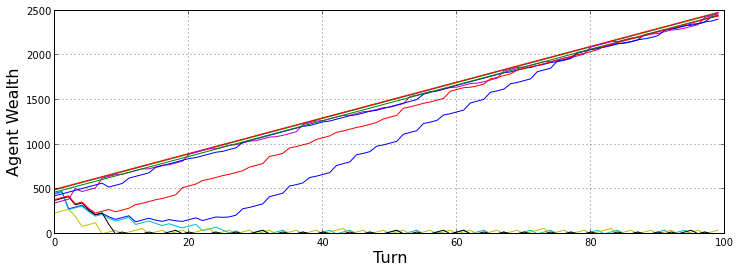
\includegraphics[width=\textwidth]{Graphics/Exp1SampleRun}
		\caption{Wealth series for all agents from representative run of heuristic model}
	\end{subfigure}

	\begin{subfigure}{0.49\textwidth}
		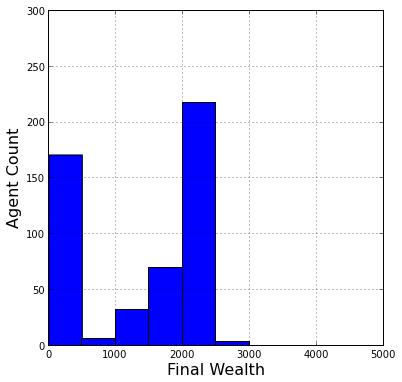
\includegraphics[width=\textwidth]{Graphics/Exp1WealthDistribution}
		\caption{Wealth distribution}
	\end{subfigure}
	\begin{subfigure}{0.49\textwidth}
		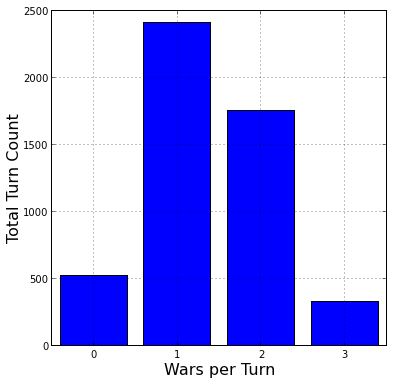
\includegraphics[width=\textwidth]{Graphics/Exp1WarDistribution}
		\caption{Wealth distribution}
	\end{subfigure}
\caption{Distribution of agent wealth and war counts across heuristic model runs}
\end{figure}

\subsection{Relative Wealth Maximization}

Figure X shows the distribution of agent wealth across all 50 of the experiment 2 models. Like the previous distribution, it is bimodal; however, it is otherwise clearly qualitatively different, with an approximately symmetric distribution around the higher-valued peak. While there may still be a core and periphery structure, the cores are more differentiated from one another.

\begin{figure}[h!]
	\centering
	\begin{subfigure}{\textwidth}
		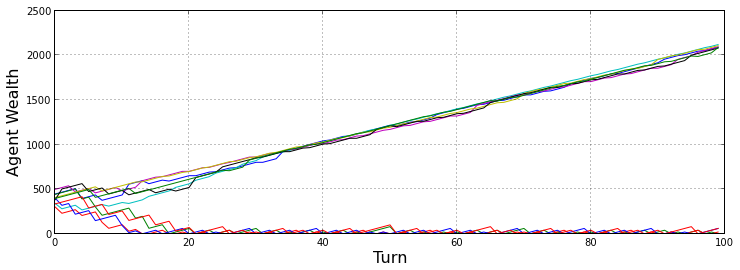
\includegraphics[width=\textwidth]{Graphics/Exp2SampleRun}
		\caption{Wealth series for all agents from representative run}
	\end{subfigure}


	\centering
	\begin{subfigure}{0.49\textwidth}
		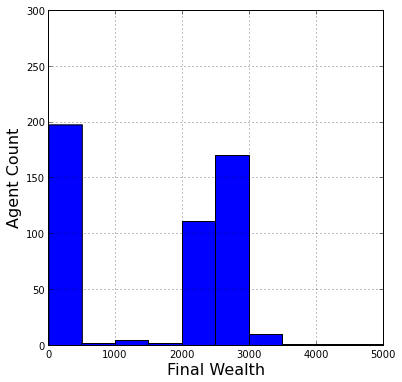
\includegraphics[width=\textwidth]{Graphics/Exp2WealthDistribution}
		\caption{Wealth distribution}
	\end{subfigure}
	\begin{subfigure}{0.49\textwidth}
		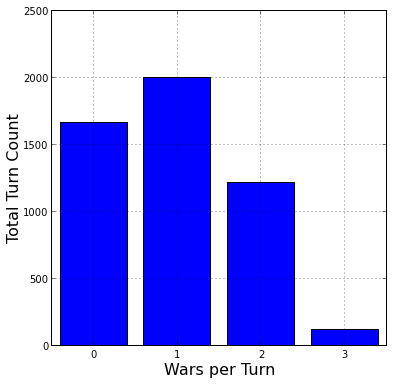
\includegraphics[width=\textwidth]{Graphics/Exp2WarDistribution}
		\caption{Wealth distribution}
	\end{subfigure}
\caption{Distribution of agent wealth and war counts across experiment 2 model runs}
\end{figure}


The distribution of war frequencies is also different, with war-free turns significantly more likely than under the heuristic. This is perhaps the clearest effect of the rational decisionmaking rule -- agents will only begin wars if they will lead to a certain, immediate relative gain, and the model confirms the intuition that they will thus engage in fewer wars overall. 

\subsection{Relative Wealth Maximization with Lookahead}

The two final experiments are similar in that they involve agents with heterogenous lookahead depths. While with experiment 3 a new interaction graph is generated for every iteration of the model, experiment 4 involves a fixed interaction graph, though the agents' initial conditions and activation sequence are randomized with every iteration. Qualitatively, both result in wealth distributions that resemble experiment 2. Note, however, that expriment 4 appears to have a tighter distribution around the upper mode, as well as a larger number of wars.

\begin{figure}[h!]
	\centering
	\begin{subfigure}{\textwidth}
		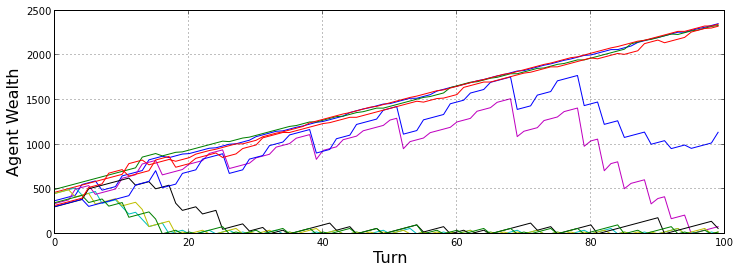
\includegraphics[width=\textwidth]{Graphics/Exp3SampleRun}
		\caption{Wealth series for all agents from representative run}
	\end{subfigure}

	\centering
	\begin{subfigure}{0.49\textwidth}
		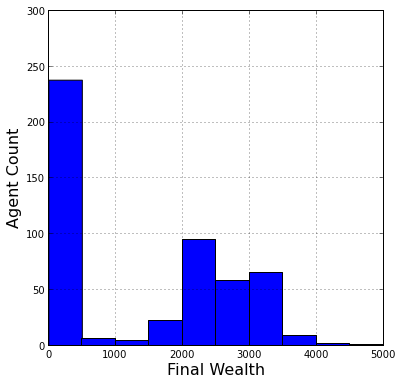
\includegraphics[width=\textwidth]{Graphics/Exp3WealthDistribution}
		\caption{Wealth distribution}
	\end{subfigure}
	\begin{subfigure}{0.49\textwidth}
		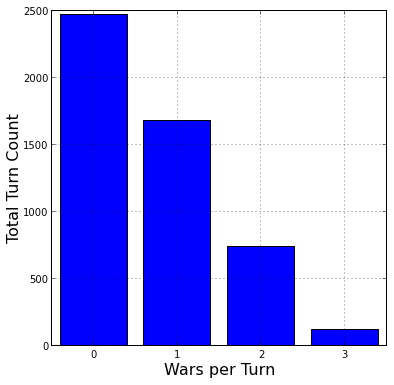
\includegraphics[width=\textwidth]{Graphics/Exp3WarDistribution}
		\caption{Wealth distribution}
	\end{subfigure}
\caption{Distribution of agent wealth and war counts across experiment 3 model runs}
\end{figure}

\begin{figure}[h!]
	\centering
	\begin{subfigure}{\textwidth}
		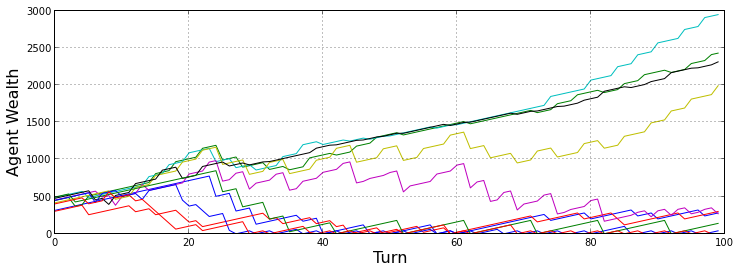
\includegraphics[width=\textwidth]{Graphics/Exp4SampleRun}
		\caption{Wealth series for all agents from representative run}
	\end{subfigure}

	\begin{subfigure}{0.49\textwidth}
		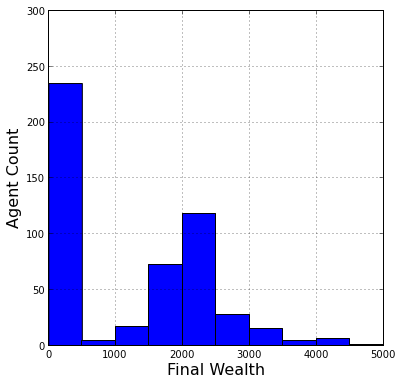
\includegraphics[width=\textwidth]{Graphics/Exp4WealthDistribution}
		\caption{Wealth distribution}
	\end{subfigure}
	\begin{subfigure}{0.49\textwidth}
		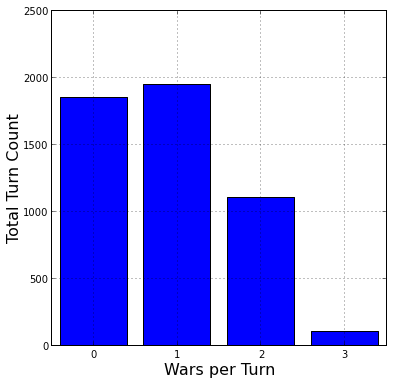
\includegraphics[width=\textwidth]{Graphics/Exp4WarDistribution}
		\caption{Wealth distribution}
	\end{subfigure}
\caption{Distribution of agent wealth and war counts across experiment 4 model runs}
\end{figure}


\subsubsection{Heterogenous Depths}

Greater recursion depth corresponds to increased intelligence, in that it allows agents to more accurately predict the decisions of the other agents further ahead. This is particularly true if agents in a model instance have heterogenous recursion depths, allowing high-depth agents to fully anticipate low-depth agents, who cannot anticipate the other agents in return. Thus, it seems reasonably to expect that when agent recursion depths are heterogenous, high-depth agents will have greater success (and achieve higher wealth) than low-depth agents. 

In order to test this hypothesis, I analyze the results of experiments 3 and 4 on an agent-by-agent basis. In addition to each agent's lookahead depth, I examine the effects of other potential factors: the agents' initial wealth, and their network degree.

I estimate these effects using a linear regression; while I have no reason to believe that the relationship is necessarily linear, this methodology should nevertheless be able to estimate the direction, magnitude and significance of the effects of each of the above characteristics on final agent wealth. 

\begin{table}
\begin{tabular}{lclcl}
\toprule
\textbf{Dep. Variable:}    &      wealth      & \textbf{  R-squared:         } &     0.041   \\
\textbf{Model:}            &       OLS        & \textbf{  Adj. R-squared:    } &     0.035   \\
\textbf{Method:}           &  Least Squares   & \textbf{  F-statistic:       } &     7.082   \\
\textbf{Date:}             & Thu, 01 May 2014 & \textbf{  Prob (F-statistic):} &  0.000114   \\
\textbf{Time:}             &     11:55:00     & \textbf{  Log-Likelihood:    } &   -4303.1   \\
\textbf{No. Observations:} &         500      & \textbf{  AIC:               } &     8614.   \\
\textbf{Df Residuals:}     &         496      & \textbf{  BIC:               } &     8631.   \\
\bottomrule
\end{tabular}

\begin{tabular}{lccccc}
\toprule
                         & \textbf{coef} & \textbf{std err} & \textbf{t} & \textbf{$P>|t|$} & \textbf{[95.0\% Conf. Int.]}  \\
\midrule
\textbf{Const.}          &    3149.0340  &      701.644     &     4.488  &      0.000     &      1770.474  4527.594      \\
\textbf{degree}          &   -1269.7681  &      297.393     &    -4.270  &      0.000     &     -1854.074  -685.462      \\
\textbf{max depth}       &      12.5764  &       37.003     &     0.340  &      0.734     &       -60.125    85.278      \\
\textbf{starting wealth} &       1.8743  &        0.973     &     1.926  &      0.055     &        -0.038     3.786      \\
\bottomrule
\end{tabular}
\caption{Regression on wealth for heterogenous recursion depth experiment}
\end{table}

\begin{table}
\begin{tabular}{lclc}
\toprule
\textbf{Dep. Variable:}    &      wealth      & \textbf{  R-squared:         } &    0.114  \\
\textbf{Model:}            &       OLS        & \textbf{  Adj. R-squared:    } &    0.109  \\
\textbf{Method:}           &  Least Squares   & \textbf{  F-statistic:       } &    21.24  \\
\textbf{Date:}             & Thu, 01 May 2014 & \textbf{  Prob (F-statistic):} & 5.83e-13  \\
\textbf{Time:}             &     12:40:42     & \textbf{  Log-Likelihood:    } &  -4214.8  \\
\textbf{No. Observations:} &         500      & \textbf{  AIC:               } &    8438.  \\
\textbf{Df Residuals:}     &         496      & \textbf{  BIC:               } &    8454.  \\
\textbf{Df Model:}         &           3      & \textbf{                     } &           \\
\bottomrule
\end{tabular}

\begin{tabular}{lccccc}
\toprule
                         & \textbf{coef} & \textbf{std err} & \textbf{t} & \textbf{$P>|t|$} & \textbf{[95.0\% Conf. Int.]}  \\
\midrule
\textbf{Const.}          &    1471.8053  &      381.695     &     3.856  &      0.000     &       721.867  2221.744      \\
\textbf{degree}          &    -591.7790  &       78.798     &    -7.510  &      0.000     &      -746.598  -436.961      \\
\textbf{max depth}       &     -18.1332  &       29.747     &    -0.610  &      0.542     &       -76.579    40.313      \\
\textbf{starting wealth} &       2.4169  &        0.845     &     2.860  &      0.004     &         0.756     4.078      \\
\bottomrule
\end{tabular}
\caption{Regression on wealth for heterogenous recursion depth with fixed graph}
\end{table}

Tables X and X show the results of these regressions for experiments 1 and 2. Both indicate similar results: the degree of an agent has a strong negative effect on its final wealth, while starting wealth has a small positive effect on it. The recursion depth, however, has essentially no effect: in both regressions, the coefficient is small and statistically insignificant. 


\section{Discussion}

The model presented here is an extremely simplified model of an international system. Unlike many previous models, its agents do not operate based on heuristics but robust adverserial search, choosing actions which maximize their relative wealth. This decision model does result in qualitative changes to the model dynamics, reducing the number and frequency of wars and increasing the variance of the distribution of agent outcomes. Nevertheless, it appears that degree of each agent's intelligence -- the depth to which it can look ahead -- does not affect its final wealth. This is an important result, for several reasons. It provides some validation for the use of simple decisionmaking heuristics, as the model behavior does not significantly diverge between the heuristic and lookahead decision rules. 

The original Axelrod model, and most other models of international systems, involve random agent activation. Implementing lookahead taking random activation into account adds several additional layers to the decisionmaking process: it would require agents to either account for all possible activation order (massively increasing the search space), or else to stochastically sample possible activations. Furthermore, facing ranges of possible outcomes, agents must weight risks and rewards, introducing implicit or explicit risk-tolerance, which may also vary between agents. However, if increased lookahead when future activations are perfectly known does not increase agent outcomes, it is unlikely to do so in the stochastic case. Instead, the stochastic elements -- both in actual activtion and internal agent forecasting -- would simply introduce noise. 

The computational resources required to implement lookahead are significant, as every agent is simulating the responses of their neighbors, those simulated agents are simulating the actions of their own neighbors, and so forth until the recursion limit is reached. The time required thus increases exponentially with each additional level of depth added. Future work may need to develop applicable pruning methods, potentially including a spatial horizon on the network beyond which agents will have a minimal effect on the currently-active agent, and thus not need to be simulated. This is important as the computational cost is what prevented this analysis from going beyond a depth of 5; it is possible that there is a qualitative shift in the effect of lookahead above a certain horizon, which has not been reached here.

The application of adversarial search algorithms into geopolitical models may yield the greatest payoff in the integration of coalitions and alliances. The original Tribute Model assumes that cooperation is deterministically driven by past interactions; the AWorld \citep{min_2003} model features a market-type mechanism for alliances, while GeoSim \citep{cederman_2003} ommits them altogether. However, \citet{russel_2009} note that cooperation may emerge endogenously from a MiniMax algorithm when the game is not zero-sum, when there are outcomes that are optimal for several agents who can cooperate to achieve it. While detailed analysis would be needed to identify instances of agent cooperation in a model run, such results would have important theoretical consequences. While the Liberal Institutionalist school of international relations often views institutionalized alliances as capable of shifting states' behaviors (as implicitly occurs in the tribute model), the Realist school \citep{mearsheimer_1995} views alliances in terms that resemble MiniMax cooperation -- as the emergent expression of states' coinciding interests. If MiniMaxing simulated political actors produce behavior resembling reality, this may be evidence that the Realist view is correct. 

More broadly, adversarial search algorithms such as the one presented here provide a powerful alternative to the heuristics generally used in geopolitical simulations to date. While qualitative theory is still needed to describe and model the system, including the agents and their utilities, adversarial search reduces the need for a qualitative theory of state decisionmaking beyond an assumption of utility maximization. Nevertheless, as this initial analysis shows, one cannot assume that `rational' actors will perform better than heuristic-driven ones.



\bibliographystyle{chicago}
\bibliography{cs580_masad}
\end{document}